\chapter{Test}

This chapter describes the tests that was done to make sure the implementation of LCS was working correctly. Also various tests was done on the test corpus using the Cosine algorithm. 

During the test segment, there was a focus on mainly four sources (their article content), those being \textit{Jyllands Posten (JP), Politiken (POL), JV.dk (JV) and \\* http://folkebladetlemvig.dk/ (FL)}. There is various reasons for picking those four. Jyllands Posten and Politiken are nation wide papers, and some of the most read in Denmark. As such, they have big budgets, big staffs and can afford doing a lot of journalistic work of their own. They could often deal with the same topics, can use the same news agencies (such as Reuters), but would often have a lot of unique material (at least that is the theory to be tested). jv.dk and folkebladetlemvig.dk are both local papers, meaning they they are only published in parts of the country. This means they to a larger extend deals with local happenings and news. They will have less focus on international material. As a small paper they will have small budgets, smaller staff and may not have the journalistic manpower to do much ground breaking, in-depth journalistic work. Also these papers are often distributed freely (their on line content may be protected by a payment wall) in the local area, and as such, their main revenue is adds sales. These adds will take up a lot of space in these papers, allowing for less news articles that in the bigger news papers. Finally a reason for picking these two sources in particular is that they are both owned by Belingske Media, and they do therefore make a good case for testing how much (if any) material is shared between media.

After doing the various implementations of the algorithms, testing was made to verify the correctness of these implementations. This interweaves with the sections of the previous chapter.

\section{Test of the basic LCS}

\begin{figure}
	\centering
	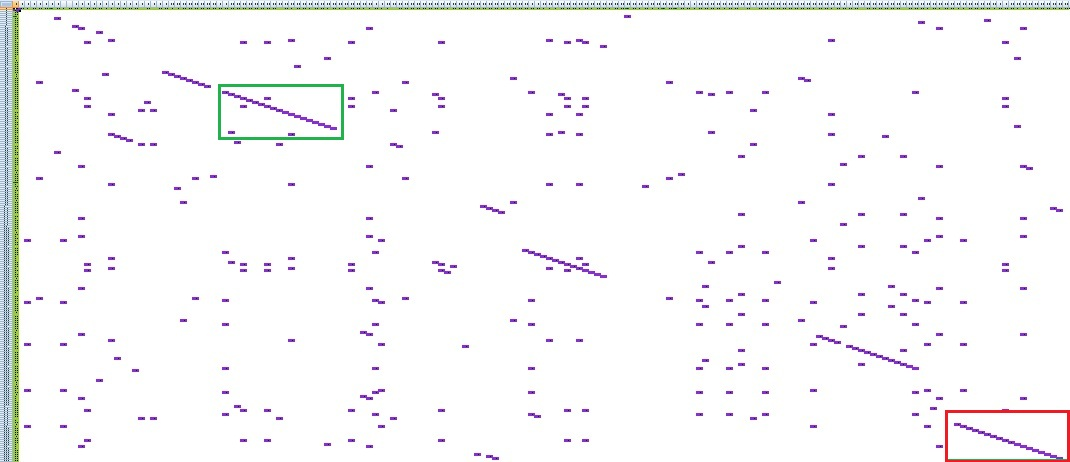
\includegraphics[scale=0.4]{figures/LcsExample}
	\caption{Diagram showing the result of two articles being compared by using LCS, and plotted in Excels. See Appendix A.1 for bigger image. The green and red boxes indicates longest common substrings found.}
	\label{LcsEx}
\end{figure}

As the final stage of the system implemented, to deal with the article duplication, there is a part that deals with post processing (see figure ~\ref{Dataflow}). This post processing mainly deals with setting up data in reader friendly way. This involves printing results to an Excel spreadsheet. Plotting the results of the LCS to a spreadsheet helps to illustrate how LCS works, and what results are being found. 

An example of this type of plot can be seen in figure~\ref{LcsEx}. The leftmost column (in green) is one article split into words, the topmost row (also in green) is another article split into words (in the basic LCS implementation the articles would be split in characters as seen in figure ~\ref{LcsExplained}). All the purple boxes indicates where a match has been found, a diagonal line indicates a row (substring) of matches. The longest one would be the \textit{'Longest Common Substring'} and the length of that would be returned by the algorithm. In the example from Figure ~\ref{LcsEx} there are two substrings of equal length (each having a length of 19 words (in the basic LCS the length would the number of characters, including white spaces)), how ever as LCS only returns the length of a single longest common substring (the longest found) and the second one (marked in the red box) is same length, LCS returns the length of the first (marked in the green box) substring. Again, as this example is made out of words rather than characters, the result could vary in case of counting actual characters, but for demonstration purposes the figure explains the idea.

In the case of a perfect match (require both articles to be of the exact same length). A line along the diagonal will be drawn. Of course the nature of representing all text in a horizontal way, distorts the image somewhat, as this makes the x-axis seem shorter than the y-axis even though the two might be of equal length. 

So, what does this image tell us? Well, for starters it shows us how LCS works. It helps us see how many words the two articles have in common, and it also helps us get an overview of how similar the two articles are, in terms of being duplicated. This was the goal of implementing the LCS in the first place.

\begin{figure}
	\centering
	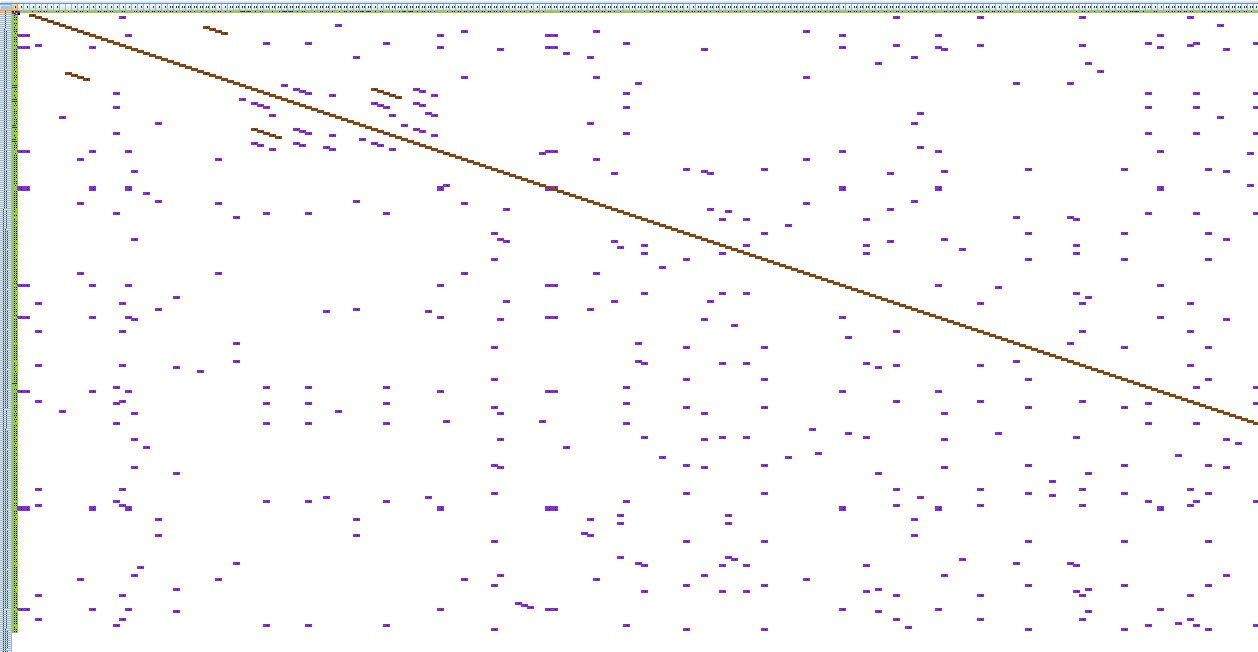
\includegraphics[scale=0.35]{figures/PerfectMatch}
	\caption{Diagram showing a part of an almost perfect match (the article along the y-axis is slightly longer than the article along the x-axis). The long brown diagonal line indicates the longest common substring found.}
	\label{Match}
\end{figure}

In Figure ~\ref{Match} there is two articles that are almost 100\% identical, the articles are from JV and FL. One of the articles ~\cite{JV1} is slightly shorter than the other article ~\cite{Lemvig1}. The on line content of the second article is protected by a payment wall, the article content can be found in Appendix B ~\ref{Levmig1:text}.
What is a added bonus of these two articles is that not only are they clearly duplicates, they are also written by the same author, \textit{Johan Winther}, who happens to be a journalist working for Berlingske Tidne\footnote{\url{http://www.b.dk/redaktionen/johan-winther}} as per 2014-05-22. This supports the thesis that the local papers, are fed news from their owning papers, to print in their own papers. This can be out of various reasons, one could be that the owning paper would have covered a story of nation wide importance, but with a special local importance. In this case, the articles deals with the company Danfoss, which is a big company in southern Jutland, and therefore has a big significance for the ares which is covered by the two local papers (JV covers southern Jutland, and FL covers the mid-west-northern part of Jutland).

\section{Test of the Modified LCS}

Once the modified version of LCS was implemented, the post processing underwent some changes to support this. The Excel printing was modified to colour the longest common substrings found, that was longer than the given threshold. All substrings that match that criteria is coloured in brown in the following. After doing some testing with the threshold, a threshold of four was selected. That value seemed to include most important sentences in terms of finding duplicates, without including too much text. Whether we remove stop words or not, should be considered when setting the threshold. Stop words are the easiest to remove or alter when modifying text, as they add little meaning to the overall topic of the text. With efficient stop removal, only key (or more significant) words will remain. These are in much higher degree a pointer to the similarity of two texts.

\begin{figure}
	\centering
	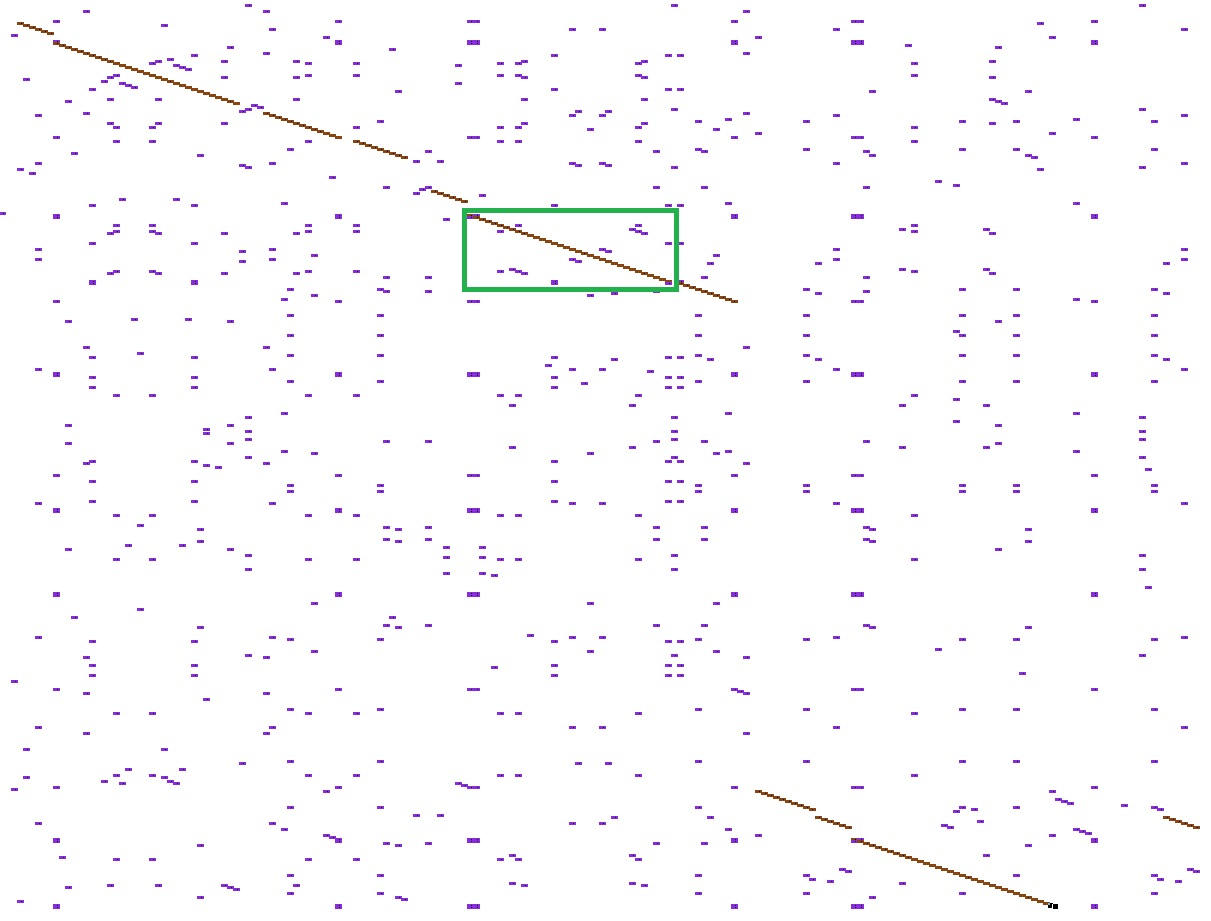
\includegraphics[scale=0.35]{figures/SubstringCollection}
	\caption{The result of having a collection of substrings). All substrings with a minimum length equal or grater to the threshold, have been coloured brown. All substrings that is short than this, is coloured in purple. If only the longest substring had been returned as the result, only the substring (marked by the brown line) in the green box would have been returned.}
	\label{SubstringsEx}
\end{figure}

As seen in figure ~\ref{SubstringsEx} the addition of substring collection significantly alters the result from what we would have gotten, had we only been using the basic LCS implementation. Judging from this diagram the two articles obviously have a lot in common. To tell if the article really have something in common it is needed to take a look at their content. The best way of doing this is by reading it the old fashion way, with your own eyes.  All of the verification done in a prototype is expected to be done this way, once the users are satisfied (through repeated manual verification) that no or only very few errors would bypass the algorithms, then the verification would be left to the algorithms (as per figure ~\ref{Architecture}).

\section{Fractile Distribution of Corpus}
The way that Consine is implemented in the inflow now, is by scoring article comparisons based on the angle between the article's vectors. This score then indicates (to some extend) how alike two articles are. The score ranges from 0.0 to 1.0. In the inflow, Infomedia simply stores all comparisons with a score above 0.6, these articles can then be verified (this is where LCS will come in handy). For this thesis however, we will compare all articles and then use the LCS on those with a Cosine score above a certain threshold. A Cosine score above 0.9 indicates, with a high degree of certainty, that the two articles being compared are practical identical (there can be modifications to this statement, will be discussed later). A certain Cosine score would therefore qualify for a comparison being automatically accepted as identical, articles below that score and down to a lower threshold would then have to controlled by human eyes. So we would like the LCS to do some of work for the humans by further cutting down the field of possible duplicates. The idea of the Cosine algorithm doing the initial splitting of article comparisons and then letting the somewhat slower LCS algorithm look into the comparisons which are uncertain in relation to being duplicates raises the following question, how many article comparisons are we looking at? For this a test of the test corpus would be made in order to give a visual representation of the task ahead.

Before setting out on the task of comparing all articles in the test corpus, a minor test was made initially. The Cosine algorithm was put to work with scoring all articles from BERL and POL sources in the test corpus, storing the results in fractiles(by intervals of 0.1), and then printing them to an Excel spreadsheet.

\begin{figure}
	\centering
	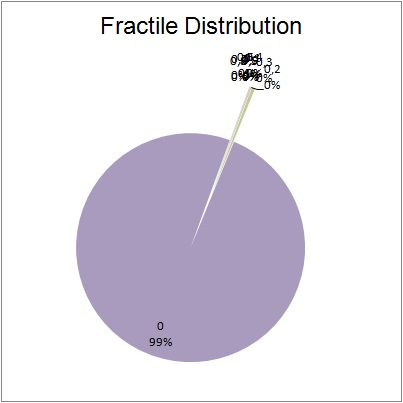
\includegraphics[scale=1.0]{figures/FractileNoise}
	\caption{The result of running Cosine on all articles in the JP and POL sources (File: "fractile noise.xlsx").}
	\label{FractileNoise}
\end{figure}

As seen in figure ~\ref{FractileNoise}, the vast majority of the article comparison are in the lowest fractile (0.0-0.1 Cosine score), and makes it really hard to use the pie chart for any sort of informative source. The scores are distributed as seen in table ~\ref{TestFractile}.

\begin{table}
\begin{center}
	\begin{tabular}{l | r}
		Cosine Score (x) & Number of Comparisons\\ \hline
		x $\leq$ 1.0 $\bigwedge$ x $\geq$ 0.9 & 2 \\ \hline
		x < 0.9 $\bigwedge$ x $\geq$ 0.8 & 1 \\ \hline
		x < 0.8 $\bigwedge$ x $\geq$ 0.7 & 0 \\ \hline
		x < 0.7 $\bigwedge$ x $\geq$ 0.6 & 1 \\ \hline
		x < 0.6 $\bigwedge$ x $\geq$ 0.5 & 2 \\ \hline
		x < 0.5 $\bigwedge$ x $\geq$ 0.4 & 8 \\ \hline
		x < 0.4 $\bigwedge$ x $\geq$ 0.3 & 9 \\ \hline
		x < 0.3 $\bigwedge$ x $\geq$ 0.2 & 17 \\ \hline
		x < 0.2 $\bigwedge$ x $\geq$ 0.1 & 98 \\ \hline
		x < 0.1 $\bigwedge$ x $\geq$ 0.0 & 21608 \\ \hline	
		Total Comparisons & 21746 \\ \hline
	\end{tabular}
\end{center}
\caption{Fractile distribution of article comparisons for JP and POL.}\label{TestFractile}
\end{table}

So in order to get a more informative view, removing the lowest fractile (comparisons scoring below 0.1 with the Cosine algorithm) will provide a better view (see figure ~\ref{NoNoise}). Please note that the value given in the various of the sections of the pie chart, is the minimum value of the fractile in question and percentage of comparisons in that fractile. The fractile named '0,9' is the fractile containing all comparisons that scored between 1.0 and 0.9(included).

\begin{figure}
	\centering
	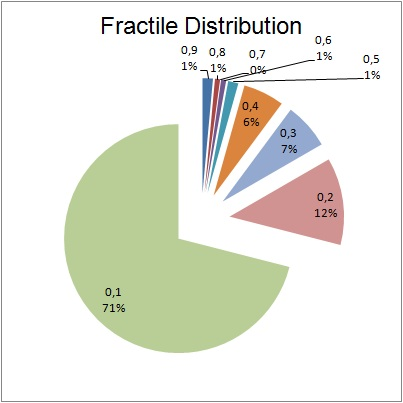
\includegraphics[scale=1.0]{figures/FractileNoNoise}
	\caption{Fractile distribution (JP and POL articles) with the comparisons scoring lower than 0.1 in the Cosine comparison removed.}
	\label{NoNoise}
\end{figure}

To double check the test result, and also to test the thesis that JV and FL do share a significant number of articles, a fractile distribution graph was made for those two sources ~\ref{JVFLFractile}.

\begin{figure}
	\centering
	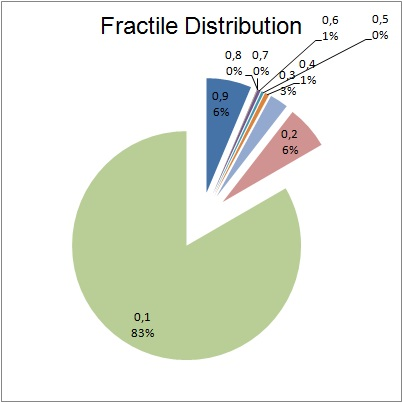
\includegraphics[scale=1.0]{figures/JVFLFractile}
	\caption{Fractile distribution (JV and FL articles) with the comparisons scoring lower than 0.1 in the Cosine comparison removed.}
	\label{JVFLFractile}
\end{figure}

\begin{table}
\begin{center}
	\begin{tabular}{l | r}
		Cosine Score (x) & Number of Comparisons\\ \hline
		x $\leq$ 1.0 $\bigwedge$ x $\geq$ 0.9 & 102 \\ \hline
		x < 0.9 $\bigwedge$ x $\geq$ 0.8 & 1 \\ \hline
		x < 0.8 $\bigwedge$ x $\geq$ 0.7 & 1 \\ \hline
		x < 0.7 $\bigwedge$ x $\geq$ 0.6 & 7 \\ \hline
		x < 0.6 $\bigwedge$ x $\geq$ 0.5 & 6 \\ \hline
		x < 0.5 $\bigwedge$ x $\geq$ 0.4 & 10 \\ \hline
		x < 0.4 $\bigwedge$ x $\geq$ 0.3 & 42 \\ \hline
		x < 0.3 $\bigwedge$ x $\geq$ 0.2 & 99 \\ \hline
		x < 0.2 $\bigwedge$ x $\geq$ 0.1 & 1342 \\ \hline
		x < 0.1 $\bigwedge$ x $\geq$ 0.0 & 53017 \\ \hline	
		Total Comparisons & 54627 \\ \hline
	\end{tabular}
\end{center}
\caption{Fractile distribution of article comparisons for JV and FL.}\label{Test2Fractile}
\end{table}


Once again we see a large amount of comparisons in the 0.1-0.2 fractile ~\ref{JVFLFractile}, it being a great deal bigger (83\% versus the 71\% in figure ~\ref{NoNoise} in the 0.1-0.2 fractile). We do however also see a bigger amount of comparisons in the top fractile (0.9-1.0) which would indicate that these two sources actually share quite a few articles, and also have more articles in common than JP and POL.

As a final test, to get the big picture of the task ahead, a test was performed for all articles in the test corpus (File: "symmetric all files fractiles.xlsx"). When running the Cosine algorithm, it is given three parameters the two first being the files to be compared, the third being a list that will contains the comparison score along with the articles information. Cosine starts with making a check of the two file sets, if they are the same, it will do a triangle comparison. This means we only have to check half the number of possible comparisons - minus the diagonal. This is handy if we want to do a comparison on a single set of articles. If you want to compare the articles from two days (or some other time frame), the algorithm will do an asymmetrical comparison, meaning that all possible comparisons are made - minus the diagonal, as checking an article with itself is trivial.

\begin{figure}
	\centering
	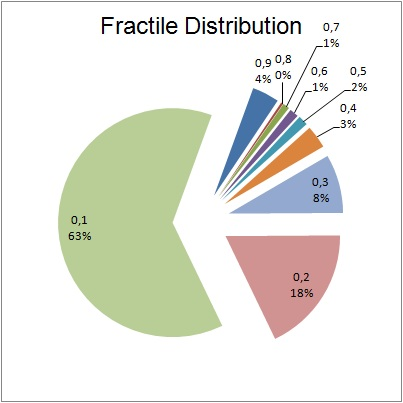
\includegraphics[scale=1.0]{figures/AllFilesFractile}
	\caption{Cosine comparison of all files in the test corpus. The fractile below 0.1 have been left out, to create a better view of the comparison distribution (File: "symmetric all files fractiles.xlsx").}
	\label{Fractles}
\end{figure}


The scores of the final test are distributed as follows (the fractile below 0.1 have been included in this table, it accounts for 99\% of the total number of comparisons) in table ~\ref{AllFractiles}.

\begin{table}
\begin{center}
	\begin{tabular}{l | r}
		Cosine Score (x) & Number of Comparisons\\ \hline
		x $\leq$ 1.0 $\bigwedge$ x $\geq$ 0.9 & 61107 \\ \hline
		x < 0.9 $\bigwedge$ x $\geq$ 0.8 & 5168 \\ \hline
		x < 0.8 $\bigwedge$ x $\geq$ 0.7 & 15090 \\ \hline
		x < 0.7 $\bigwedge$ x $\geq$ 0.6 & 20443 \\ \hline
		x < 0.6 $\bigwedge$ x $\geq$ 0.5 & 22472 \\ \hline
		x < 0.5 $\bigwedge$ x $\geq$ 0.4 & 51945 \\ \hline
		x < 0.4 $\bigwedge$ x $\geq$ 0.3 & 132699 \\ \hline
		x < 0.3 $\bigwedge$ x $\geq$ 0.2 & 286529 \\ \hline
		x < 0.2 $\bigwedge$ x $\geq$ 0.1 & 1001151 \\ \hline
		x < 0.1 $\bigwedge$ x $\geq$ 0.0 & 247311986 \\ \hline	
		Total Comparisons & 248908590 \\ \hline
	\end{tabular}
\end{center}
\caption{Fractile distribution for all files compared in Cosine.} \label{AllFractiles}
\end{table}

As table ~\ref{AllFractiles} shows, there is a massive amount of comparisons in the lowest fractile (close to quarter of a billion comparisons, the total number of comparisons above that is approximately 1,6 million comparisons (1,596,604 comparisons).

After doing these test, it would seem like the various parts of the project is working as planned, and it is now time to evaluate the results produced by running the program.
